% 2008 年浙江卷理科第 10 题：AB 是平面 α 的斜线段，A 为斜足，P 在平面 α 内运动，
%   使 △ABP 的面积为定值。
% 来源 PDF：gaokaomath-src/普通高考/2008/2008浙江理.pdf
% SHA-256：61b86d188443ba25020577365e293aa0999ec32fb32b9791690cec6ac85cf0db
% 原页：2008浙江理.pdf 第 1 页（A3 三栏）第 1 栏，书页码 491。
% 重绘依据：平面 α 画成平行四边形，B 在平面上方，A 为平面内的斜足（与 B 的射影 H 分开），
%   P 在平面内右侧；BA、BP、AP 实线，B 到平面的垂线 BH 为虚线。
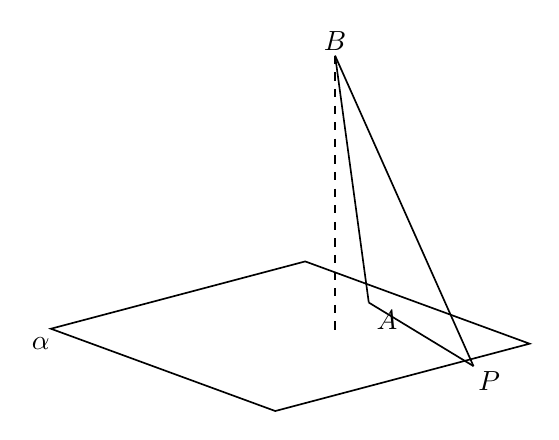
\begin{tikzpicture}[scale=0.95, semithick, every node/.style={inner sep=1.5pt}]
  % 平面 α
  \draw (-2.2,-0.45) -- (0.8,-1.55) -- (4.2,-0.65) -- (1.2,0.45) -- cycle;
  \node[below left] at (-2.15,-0.5) {$\alpha$};

  \coordinate (B) at (1.60,3.20);
  \coordinate (H) at (1.60,-0.55);
  \coordinate (A) at (2.05,-0.10);
  \coordinate (P) at (3.45,-0.95);

  \draw (B) -- (A);
  \draw (B) -- (P);
  \draw (A) -- (P);
  \draw[dashed] (B) -- (H);

  \node[above] at (B) {$B$};
  \node[below right=1pt] at (A) {$A$};
  \node[below right] at (P) {$P$};
\end{tikzpicture}
